\documentclass{classrep}
\usepackage[utf8]{inputenc}
\frenchspacing

\usepackage{graphicx}
\usepackage[usenames,dvipsnames]{color}
\usepackage[hidelinks]{hyperref}
\usepackage{lmodern}
\usepackage{placeins}
\usepackage{url}
\usepackage{amsmath, amssymb, mathtools}
\usepackage{listings}
\usepackage{fancyhdr, lastpage}
\usepackage{subfiles}

\pagestyle{fancyplain}
\fancyhf{}
\renewcommand{\headrulewidth}{0pt}
\cfoot{\thepage\ / \pageref*{LastPage}}

\definecolor{codegreen}{rgb}{0,0.6,0}
\definecolor{codegray}{rgb}{0.5,0.5,0.5}
\definecolor{codepurple}{rgb}{0.58,0,0.82}
\definecolor{backcolour}{rgb}{0.95,0.95,0.92}

\lstdefinestyle{mystyle}{
    commentstyle=\color{codegreen},
    keywordstyle=\color{magenta},
    numberstyle=\tiny\color{codegray},
    stringstyle=\color{codepurple},
    basicstyle=\ttfamily\footnotesize,
    breakatwhitespace=false,
    breaklines=true,
    captionpos=b,
    keepspaces=true,
    numbers=left,
    numbersep=5pt,
    showspaces=false,
    showstringspaces=false,
    showtabs=false,
    tabsize=2
}

\lstset{style=mystyle}

%--------------------------------------------------------------------------------------%
\studycycle{Informatyka stosowana, studia dzienne, II st.}
\coursesemester{II}

\coursename{Eksploracja danych internetowych}
\courseyear{2021/2022}

\courseteacher{dr inż. Krzysztof Myszkorowski}
\coursegroup{poniedziałek, 12:15}

\author{%
    \studentinfo[239671@edu.p.lodz.pl]{Jan Karwowski}{239671}\\
    \studentinfo[239676@edu.p.lodz.pl]{Kamil Kowalewski}{239676}\\
}

\title{Zadanie 2.: Analiza atrybutów i klastrowa stron internetowych}

\begin{document}
    \maketitle
    \thispagestyle{fancyplain}

    \tableofcontents
    \newpage

    \section{Cel}
    \label{purpose} {
        Celem zadania było dokonanie analizy atrybutów oraz analizy klastrowej dokumentów
        z wybranych stron internetowych. Na każdym ze źródłem HTML wybranych stron
        internetowych nalezało dokonać transformacji celem przekształcenia zawartości
        HTML na postać pliku tekstowego. Kolejnym krokiem była analiza atrybutów
        dokumentów w zależności od reprezentacji oraz parametrów konfiguracyjnych
        programu Weka\cite{weka}. Krok, który został wykonany jako następny była
        klasteryzacja tych dokumentów dla każdego przypadku. Przechodząc do stron
        wykorzystanych do analizy są to kolejno:

        \begin{itemize}
            \item https://ftims.p.lodz.pl/
            \item http://www.weeia.p.lodz.pl/
        \end{itemize}
    }

    \section{Przygotowanie plików z danymi} {
        Aby zebrać dane ze stron internetowych oraz ich podstron, które zostały
        wymienione w sekcji \ref{purpose}, zostało wykorzystane oprogramowanie typu
        \textit{Web Crawler} o nazwie \textit{WebSPHINX}\cite{websphinx}.

        Następnym krokiem było dokonanie ekstrakcji tekstu czyli wyłuskanie zawartości
        jaki widzi użytkownik poprzez usunięcie wszystkich elementów HTML. Do tego celu
        został stworzony program w języku Python posiadający dwa tryby działania. Tryb,
        który jest potrzebny w tym procesie jest to \textit{python main.py --plain},
        jego działanie opiera się na wykorzystaniu biblioteki
        \emph{html2text}\cite{html2text}.

        Drugim trybem działania uruchamianym przez \textit{python main.py --arff} jest
        wytworzenie pliku o rozszerzeniu \textit{.arff}, który jest wymagany przez
        program Weka\cite{weka}. Sam plik zawiera pogrupowane podstrony z zachowanym
        schematem dwóch atrybutów
        \begin{itemize}
            \item title - tytuł strony
            \item content - zawartość strony
        \end{itemize}
        którego przykład został przestawiony poniżej:

    % @formatter:off
        \begin{lstlisting}
@relation index
@attribute title string
@attribute content string
        \end{lstlisting}
    % @formatter:on
    }

    \section{Metody przeprowadzenia badań} {

        \subsection{Analiza atrybutów} {
            Przed każdorazowym dokonaniem analizy atrybutów był uruchamiany filtr
            \emph{weka.filters.unsupervised.attribute.StringToNominal}, którego
            konfiguracja został przedstawiona na rysunku \ref{string_to_nominal_setup}.

            \begin{figure}[!htbp]
                \centering
                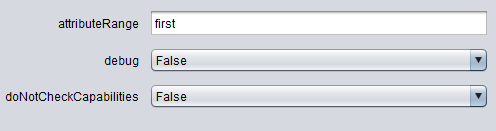
\includegraphics[width=0.8\textwidth]{img/string_to_nominal_setup.png}
                \caption{Ustawienia filtru StringToNominal}
                \label{string_to_nominal_setup}
            \end{figure}
            \FloatBarrier

            Następnie został wykorzystany filtr \textit{StringToWordVector} i za pomocą
            niego były konfigurowane warianty eksperymentów poprzez zmiany parametrów
            outputWordCounts, StopwordsHandler, TFTransform, IDFTransform w różnych
            kombinacjach. Kombinacje te zostały przedstawione w formie tabeli w każdej
            z podsekcji z eksperymentami.
        }

        \subsection{Analiza klastrowa} {
            Do analizy klastrowej został wykorzystany algorytm EM
            (ang. Expectation–Maximization), który jest interacyjną metodą szacowania
            maksymalnego prawdopodobieństwa. Wykonuję on dwa kroki, pierwszy z nich to
            wyznaczenie wartości spodziewanego prawdopodobieństwa oraz drugi z nich to
            obliczenie rozkładu parametrów oraz wiarygodności zmiennych. Trwa to
            iteracyjnie do momentu osiągniecia maksymalnej wartości wiarygodności.
            Kluczową jego zaleta w przypadku tego użycia jest to, że nie trzeba podawać
            liczby klastrów. Był on wykorzystywany dla parametrów przedstawiony na
            rysunku \ref{em_setup}

            \begin{figure}[!htbp]
                \centering
                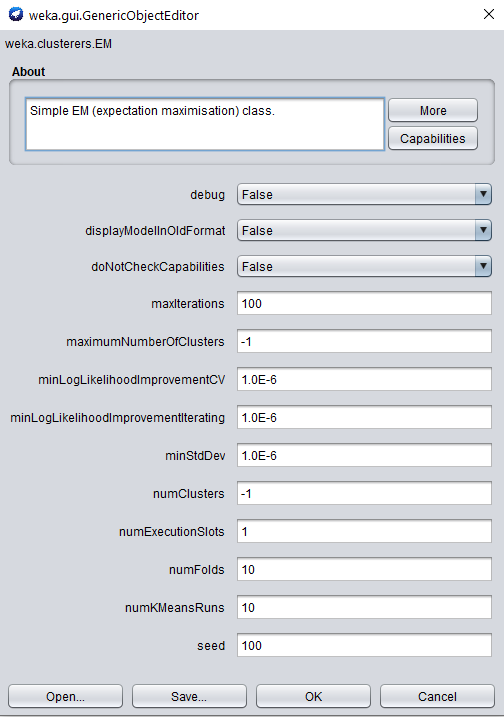
\includegraphics[width=0.8\textwidth]{img/em-setup.png}
                \caption{Parametry algorytmu EM}
                \label{em_setup}
            \end{figure}
            \FloatBarrier
        }
    }
    \newpage

    \section{Wyniki dla domeny \textit{https://ftims.p.lodz.pl/}} {
        \subfile{section/results1.tex}
    }
    \newpage

    \section{Wyniki dla domeny \textit{http://www.weeia.p.lodz.pl/}} {
        \subfile{section/results2.tex}
    }

    \section{Dyskusja} {

        \subsection{Analiza atrybutów} {
            Dla dwóch domen i przypadków numer 1,3,8 uzyskano zbliżone wyniki, gdyż są
            to macierze binarne co przekazuję bardzo mało informacji. Dla przypadku
            numer 2 czy z wykorzystaniem outputWordCount rozszerza wcześniej wspomniane
            podpunktu o liczbę wystąpień danego słowa. Dla przypadku 4 - TFTransform
            oraz przypadku 5 - IDFTransform zostały zwrócone znacznie bardziej
            wartościowe wyniki ponieważ biorą pod uwagę kontekst całego dokumnentu oraz
            inne dokumenty poddawane analizie. Złączenie ich w TFIDF daję już naprawdę
            ciekawe wyniki, pozwala ono na odfiltrowywanie popularnych terminów. Aby
            uzyskać wysoką wagę TFIDF muszą być spełnione dwa warunki, pierwszym z nich
            jest wysoka częstotliwość terminów w danym dokumencie oraz mała częstości
            występowania tego terminu w pozostałych dokumentach. Im wyższa wartość
            liczbowa wagi tym rzadszy termin.
        }

        \subsection{Analiza klastrowa} {
            Po dokonaniu analizy klastrowej dla domeny \textit{https://ftims.p.lodz.pl/}
            dla przypadków numer 1 (bazowy), 4 (TF), 5 (IDF), 6 (TFIDF) uzyskano 6
            klastrów o dokładnie takim samym rozkładzie procentowym. Dla przypadków
            7 (TFIDF + outputWordCounts) oraz 8 (reprezentacja binarna) uzyskano również
            6 klastrów natomiast liczności klastrów były dosyć mocno zróżnicowane.
            Analiza przypadków numer 2 (outputWordCounts) oraz 3 (StopwordsHandler)
            przyniosła dużo bardziej zróżnicowane wyniki niż w w/w eksperytmenty gdzie
            maksymalna liczności jednego klastra nie przekraczała \textit{40\%}, dla
            przypadku numer 2 został utworzony jeden klaster zawierający \textit{100\%}
            natomiast dla przypadku numer 3 zostały utworzone 3 klastry z tego są dwa
            dominujące zawierające odpowiednio \textit{67\%} oraz \textit{29\%}.

            Analiza klastrowa domeny \textit{http://www.weeia.p.lodz.pl/} dała inne
            rezultaty. Dla przypadków 1 (bazowy) i 4 (TF) uzyskano identyczne wyniki,
            zostały utworzone 4 klastry, gdzie jeden z nich był mocno dominujący gdyż
            posiadał aż \textit{69\%}. Kolejną grupą były przypadki 5 (IDF), 6 (TFIDF)
            oraz 7 (TFIDF + outputWordCounts), gdzie utworzono 5 klastrów i znów jeden
            z nich był mocno dominujący gdyż posiadał w sobie aż \textit{80\%} próbek.
            Dla przypadku numer 7 jedynie kolejność mniejszych klastrów była różna od
            tych dla przypadków numer 5 i 6. Dla przypadków 2 (outputWordCounts),
            3 (StopwordsHandler) oraz 8 (reprezentacja binarna) uzyskano odpowiednio
            następujące liczby klastrów 12, 4, 3 gdzie w każdym przypadku występuję
            dominujący klaster zawierający ponad \(\frac{2}{3}\) próbek.

            Porównując wyniki uzyskane dla w/w domen można stwierdzić, że te dla
            \textit{https://ftims.p.lodz.pl/} są znacznie ciekawsze gdyż, zmieniając
            parametry uzyskiwaliśmy rozkład zazwyczaj na dwa lub trzy wysokoliczne
            klastry, które rozkłady procentowe różniły sie od siebie. Dla drugiej
            domeny a mianowicie \textit{http://www.weeia.p.lodz.pl/} zawsze był
            generowany jeden duży klaster a liczba powstałych klastrów małolicznych
            była zależna od uruchomienia danego parametru.
        }
    }

    \begin{thebibliography}{0}
        \bibitem{weka}{https://www.cs.waikato.ac.nz/ml/weka/}
        \bibitem{websphinx}{https://www.cs.cmu.edu/~rcm/websphinx/}
        \bibitem{html2text}{https://pypi.org/project/html2text/}
    \end{thebibliography}

\end{document}
